\begin{tcolorbox}[colback=red!3!white,colframe=red!50!black,boxrule=0.8pt,title={Korrekturhinweise},fonttitle=\bfseries]
\textbf{Korrekturen aus der Rechenprüfung (30.~Sept.~2026).} Die folgenden Stellen sind im Text korrigiert bzw. vermerkt; jede trägt dort einen datierten Hinweis mit dem vorherigen Wert (die Einordnung der Myon-Anomalie regelt der Hinweis zu Dok.~382):
\begin{itemize}
\item Vergleich mit alternativen Theorien: $138{,}93\times0{,}9862 = 137{,}036 \to 137{,}01$; Weitere Bezüge: $K_{\text{frak}} = 0{,}9862$ stammt aus dem älteren Anker $D_f = 2{,}94$ (vermerkt).
\item Vergleich mit dem Experiment: theoretisches $m_\mu/m_e$ $206{,}768$ (Messwert) $\to \frac{12}{5}\xi^{-1/2} = 207{,}85$.
\item Tabelle 22.1.1: $c_e$-Mantisse $= e \to \sqrt e$; Abschnitt 19: ausgegebene Massen sind Messwerte (Anker), mit gemeinsamem Anker nicht erreichbar (vermerkt).
\item Box 11.6.1: $\alpha = \frac{m_e m_\mu}{7500}\times0{,}986 \to \frac{m_e m_\mu}{7500\times0{,}986}$ ($K_{\text{frak}}$ wirkt auf $\alpha^{-1}$); geboxte $\alpha$-Formel (3.6.1, 9.3.1, 23.9.1) ergibt $2{,}4\times10^{-9}$, $K_{\text{frak}}$ gehört zu $\alpha^{-1}$ (vermerkt).
\item Massenverhältnisse: $c_\mu/c_e = 3\sqrt3/(2\sqrt\alpha) \to \sqrt3/(2\sqrt\alpha)$, ergibt $m_\mu/m_e \approx 878$.
\item Abschnitt 11.3.2: $138{,}91\times0{,}986 = 137{,}04 \to 136{,}97$.
\item Tau-Masse 4.2.3: $\frac54\xi^{2/3}\cdot246$~GeV $= 1{,}777 \to 0{,}80$~GeV.
\item Abschnitt 23.5/23.6: $\alpha \approx 7{,}292\times10^{-3}$, $\alpha^{-1} \approx 137{,}13 \to \alpha \approx 2{,}42\times10^{-9}$ ($0{,}5923^{0{,}4} = 0{,}8110$, $\xi^{2{,}2} = 2{,}984\times10^{-9}$).
\item Abschnitt 23.8.1: $138{,}949\times0{,}9862 = 137{,}036 \to 138{,}911\times0{,}9862 = 136{,}99$.
\item Abschnitt 10.1: $\alpha = m_e m_\mu/7380$ mit $7380 = 7500/K_{\text{frak}}$ ($= 7605$) $\to m_e m_\mu/7400$, $7400 = 7500\,K_{\text{frak}}$ ($\alpha^{-1} = 137{,}06$).
\item Abschnitte 12.5 und 16.2.5: $\xi^{11/2} = 5{,}19\times10^{-22} \to 4{,}87\times10^{-22}$, $1{,}4\times10^{19} \to 1{,}5\times10^{19}$.
\item Abschnitt 3.2.2: gravitativ-geometrische Herleitung $\Ezero^2 = 4\sqrt2\,m_\mu/\xipar^4$ ($1{,}4\times10^{9}$~MeV) entfernt $\to$ $\sqrt{m_e m_\mu/K_{\text{frak}}}$.
\item Abschnitt 13.7.1: \enquote{passen zu $m_\mu/m_e \approx 207$} $\to$ ergeben $m_\mu/m_e \approx 878$; 14.1.1 und 18.1.1--18.3.1: angegebene Koeffizientenwerte folgen nicht aus den Formeln (vermerkt).
\item Abschnitt 2.2: $\Ezero = \frac34\times10^4\,\EP$ widerspricht $\Ezero = 7{,}398$~MeV (vermerkt); Hierarchietabelle: $m_\tau/m_\mu$ aus $y_\tau/y_\mu$ $\sim17 \to 5{,}73$; 14.3.1: $m^{\text{nat}} = m^{\text{SI}}G/(\hbar c) \to m^{\text{SI}}\sqrt{G/(\hbar c)}$, $\xi$ ohne Umrechnung; 16.3.1: \enquote{Planck-Energie zu Elektronenvolt} $\to$ zu GeV; 20.1.1: $\sqrt{c_e c_\mu}\,\xi^{9/4} = 5{,}9\times10^{-8}$, nicht $7{,}346881$~MeV (vermerkt); Tabelle 22.1.1: $\xi^{5/2} = 3{,}098\times10^{-10} \to 2{,}0528\times10^{-10}$; $E_0^{\text{korr}} = K_{\text{frak}}E_0^{\text{bare}}$ widerspricht R72 (vermerkt).
\item (2.~Okt.~2026) Bezeichnung $f$: allgemeine Abhängigkeit $\alpha = f(\xi)$ --- keine Frequenz; Vermerk im Text (Dok.~190, R147).
\end{itemize}

\medskip\noindent\textbf{Hinweis zum Stand Myon $g-2$ (2025).} Dieses Dokument bezieht sich auf die Abweichung zwischen gemessenem $a_\mu$ und der Standardmodell-Vorhersage, wie sie 2021 vorlag. Mit dem Fermilab-Endergebnis und dem White Paper~2025 der Muon~$g-2$ Theory Initiative ist diese Abweichung nicht mehr signifikant. Aussagen, die die Anomalie als Beleg oder als Zielgröße eines T0-Beitrags verwenden, sind überholt; den aktuellen Stand und die Einordnung gibt Dok.~382.
\end{tcolorbox}

\section*{Zur mathematischen Struktur der T0-Theorie: Warum Zahlenverhältnisse nicht direkt gekürzt werden dürfen}

	\medskip\noindent\textbf{Hinweis zur Fassung.} Die deutsche und die englische Fassung dieses Dokuments weichen in Aufbau und Umfang voneinander ab; bei früheren Überarbeitungen wurden in beiden Fassungen Teile gekürzt, ergänzt oder anders gefasst. Bei Abweichungen gilt die umfangreichere deutsche Fassung; Abschnitte, die nur die englische Fassung enthält, gelten als Ergänzung.

	
	\medskip\noindent\textbf{Statusmarker.} Aussagen mit \textbf{[S]} sind \emph{spekulativ}: ein Hinweis oder eine Vermutung, die im Korpus noch nicht hergeleitet oder numerisch geprüft ist.

	
	\subsection*{Einleitung}
	
	In der theoretischen Physik stellt sich oft die Frage, welche mathematischen Operationen legitim sind und welche nicht. Ein besonders interessantes Problem tritt in der T0-Theorie auf, wo scheinbar einfache Zahlenverhältnisse wie $\frac{2}{3}$ und $\frac{8}{5}$ eine tiefere strukturelle Bedeutung besitzen, die ein direktes Kürzen verbietet.
	
	\subsection*{Das fundamentale Problem}
	
	Die T0-Theorie postuliert zwei äquivalente Darstellungen für die Leptonenmassen:
	
	\begin{align*}
		\textbf{Einfache Form:} &\quad m_e = \frac{2}{3} \cdot \xi^{5/2}, \quad m_\mu = \frac{8}{5} \cdot \xi^2 \\
		\textbf{Erweiterte Form:} &\quad m_e = \frac{3\sqrt{3}}{2\pi\alpha^{1/2}} \cdot \xi^{5/2}, \quad m_\mu = \frac{9}{4\pi\alpha} \cdot \xi^2
	\end{align*}
	
	Auf den ersten Blick könnte man annehmen, dass die Brüche $\frac{2}{3}$ und $\frac{8}{5}$ einfache rationale Zahlen sind, die man kürzen oder vereinfachen könnte. Doch diese Annahme wäre falsch.
	
	\subsection*{Warum direktes Kürzen nicht erlaubt ist}
	
	Die Gleichsetzung beider Darstellungen führt zu:
	
	\[
	\frac{2}{3} = \frac{3\sqrt{3}}{2\pi\alpha^{1/2}}, \quad \frac{8}{5} = \frac{9}{4\pi\alpha}
	\]
	
	Diese Gleichungen zeigen, dass die scheinbar einfachen Brüche in Wirklichkeit zusammengesetzte Ausdrücke sind, die Konstanten ($\pi$, $\alpha$) und geometrische Faktoren ($\sqrt{3}$) enthalten.
	
	\subsection*{Mathematische und physikalische Konsequenzen}
	
	\begin{enumerate}
		\item \textbf{Struktur-Erhaltung}: Das direkte Kürzen würde die zugrundeliegende geometrische und physikalische Struktur zerstören.
		
		\item \textbf{Informationverlust}: Die Brüche codieren Information über die Raumzeit-Geometrie und die elektromagnetische Kopplung.
		
		\item \textbf{Äquivalenz-Prinzip}: Beide Darstellungen sind mathematisch äquivalent, aber die erweiterte Form enthüllt den physikalischen Ursprung.
	\end{enumerate}
	
	\section{Zirkuläre Verhältnisse und fundamentale Konstanten}
\label{sec:zirkulaer}

In der T0-Theorie kommt es zu scheinbar zirkulären Verhältnissen, die jedoch Ausdruck der Verknüpfung der Konstanten im T0-Rahmen sind:

\begin{align*}
	\alpha &= f(\xi) \\
	\xi &= g(\alpha)
\end{align*}

\textit{(Vermerk vom 2.~Okt.~2026 zur Bezeichnung: $\alpha = f(\xi)$ ist hier eine allgemeine Abhängigkeit, keine Frequenz und nicht die Grundwindungszahl $f = 1/\xi$. Vgl.\ Dok.~190, R147.)}

Diese wechselseitige Abhängigkeit führt zu einem scheinbaren Henne-Ei-Problem: Was kommt zuerst, $\alpha$ oder $\xi$?

\subsection{Lösung des Zirkularitätsproblems}

Die Lösung liegt in der Erkenntnis, dass beide Konstanten Ausdruck einer zugrundeliegenden geometrischen Struktur sind:

\begin{tcolorbox}[colback=green!5!white,colframe=green!75!black]
	\textbf{$\alpha$ und $\xi$ sind nicht unabhängig voneinander, sondern emergente Eigenschaften der fraktalen Raumzeit-Geometrie.}
\end{tcolorbox}

Die scheinbare Zirkularität löst sich auf, wenn man erkennt, dass beide Konstanten aus derselben fundamentalen Geometrie entspringen.

\section{Die Rolle natürlicher Einheiten}
\label{sec:einheiten}

In natürlichen Einheiten setzen wir konventionsgemäß $\alpha = 1$ für bestimmte Berechnungen. Dies ist legitim, weil:

\begin{itemize}
	\item Die fundamentale Physik unabhängig von Maßeinheiten sein sollte
	\item Dimensionslose Verhältnisse die eigentlichen physikalischen Aussagen enthalten
	\item Die Wahl $\alpha = 1$ eine spezielle Eichung darstellt
\end{itemize}

Allerdings darf diese Konvention nicht darüber hinwegtäuschen, dass $\alpha$ in der T0-Theorie einen bestimmten numerischen Wert hat, der durch $\xi$ bestimmt wird.

\begin{tcolorbox}[colback=blue!5!white,colframe=blue!75!black]
	\textbf{Die scheinbar einfachen Zahlenverhältnisse in der T0-Theorie sind nicht willkürlich gewählt, sondern repräsentieren komplexe physikalische Zusammenhänge.} \\
	
	Das direkte Kürzen dieser Verhältnisse wäre mathematisch zwar möglich, physikalisch aber falsch, da es die zugrundeliegende Struktur der Theorie zerstören würde. Die erweiterte Form zeigt, woher diese scheinbar einfachen Brüche im T0-Rahmen stammen, und macht ihre Verbindung zu $\pi$, $\alpha$ und geometrischen Faktoren sichtbar.
	
	Die scheinbare Zirkularität zwischen $\alpha$ und $\xi$ ist Ausdruck ihrer gemeinsamen geometrischen Herkunft und kein logisches Problem der Theorie.
\end{tcolorbox}

	% Abschnitt 1: Grundlage
	\section{Grundlage: Die einzige geometrische Konstante}
	
	\subsection{Der universelle geometrische Parameter}
	
	\noindent \textbf{1.1.1} Die T0-Theorie beginnt mit einer einzigen dimensionslosen Konstante, die aus der Geometrie des dreidimensionalen Raums motiviert ist:
	
	\begin{keyresult}
		\begin{equation}
			\boxed{\xipar = \frac{4}{3} \times 10^{-4}}
		\end{equation}
	\end{keyresult}
	
	\noindent \textbf{1.1.2} Diese Konstante ergibt sich aus:
	\begin{itemize}
		\item Der tetraedrischen Packungsdichte des 3D-Raums: $\frac{4}{3}$
		\item Der Skalenhierarchie zwischen Quanten- und klassischen Bereichen: $10^{-4}$ (motivierte Setzung des Exponenten)
	\end{itemize}
	
	\subsection{Natürliche Einheiten}
	
	\noindent \textbf{1.2.1} Wir arbeiten in natürlichen Einheiten, wobei:
	\begin{align}
		c &= 1 \quad \text{(Lichtgeschwindigkeit)} \\
		\hbar &= 1 \quad \text{(reduzierte Planck-Konstante)} \\
		G &= 1 \quad \text{(Gravitationskonstante, numerisch)}
	\end{align}
	
	\noindent \textbf{1.2.2} Die Planck-Länge dient als Referenzskala:
	\begin{equation}
		\lP = \sqrt{G} = 1 \quad \text{(in natürlichen Einheiten)}
	\end{equation}
	
	% Abschnitt 2: Aufbau der Skalenhierarchie
	\section{Aufbau der Skalenhierarchie}
	
	\subsection{Schritt 1: Charakteristische T0-Skalen}
	
	\noindent \textbf{2.1.1} Aus $\xipar$ und der Planck-Referenz leiten wir die charakteristischen T0-Skalen ab:
	\begin{align}
		\rzero &= \xipar \cdot \lP = \frac{4}{3} \times 10^{-4} \cdot \lP \\
		\tzero &= \rzero = \frac{4}{3} \times 10^{-4} \quad \text{(in Einheiten mit } c=1\text{)}
	\end{align}
	
	\subsection{Schritt 2: Energieskalen aus Geometrie}
	
	\noindent \textbf{2.2.1} Die charakteristische Energieskala ergibt sich aus der Dimensionsanalyse:
	\begin{equation}
		\Ezero = \frac{1}{\rzero} = \frac{3}{4} \times 10^{4} \quad \text{(in Planck-Einheiten)}
	\end{equation}
	
	\noindent \textbf{2.2.2} Dies ergibt die T0-Energiehierarchie:
	\begin{align}
		\EP &= 1 \quad \text{(Planck-Energie)} \\
		\Ezero &= \xipar^{-1} \EP = \frac{3}{4} \times 10^{4} \EP
	\end{align}
	\textit{(Vermerk vom 30.~Sept.~2026: $\Ezero = \xipar^{-1}\EP = 7500\,\EP = 9{,}2\times10^{22}$~GeV widerspricht $\Ezero = 7{,}398$~MeV in Abschnitt~3; mit diesem $\Ezero$ wäre $\xipar\Ezero^2 = 1/\xipar = 7500$, nicht $\alpha$. Die Gleichsetzung $\Ezero = 1/\rzero$ in Planck-Einheiten ist mit der übrigen Herleitung nicht vereinbar.)}
	
	% Abschnitt 3: Ableitung der Feinstrukturkonstanten
	\section{Ableitung der Feinstrukturkonstanten}
	
	\subsection{Ursprung der Formel $\varepsilon = \xipar \cdot \Ezero^2$}
	
	\noindent \textbf{3.1.1} Die fundamentale Formel der T0-Theorie für den Kopplungsparameter $\varepsilon$ lautet:
	\begin{keyresult}
		\begin{equation}
			\boxed{\varepsilon = \xipar \cdot \Ezero^2}
			\label{eq:epsilon_definition}
		\end{equation}
	\end{keyresult}
	
	\noindent \textbf{3.1.2} Diese Beziehung verbindet:
	\begin{itemize}
		\item $\varepsilon$ -- der T0-Kopplungsparameter
		\item $\xipar$ -- der geometrische Parameter aus der Tetraeder-Packung
		\item $\Ezero$ -- die charakteristische Energie
	\end{itemize}
	
	\subsection{Die charakteristische Energie $\Ezero$}
	
	\noindent \textbf{3.2.1} Die charakteristische Energie $\Ezero$ ist definiert als das geometrische Mittel der Elektron- und Myonenmasse:
	\begin{equation}
		\Ezero = \sqrt{m_e \cdot m_\mu}
		\label{eq:E0_geometric_mean}
	\end{equation}
	
	\noindent \textbf{3.2.2} Mit der fraktalen Korrektur (Dok.~190, R72) wird daraus:
	\begin{equation}
		\Ezero = \sqrt{\frac{m_e \cdot m_\mu}{K_{\text{frak}}}}
	\end{equation}
	
	\noindent \textbf{3.2.3} Nackt und fraktal korrigiert ergibt sich:
	\begin{equation}
		\Ezero = 7.348 \text{ MeV (nackt)}, \qquad \Ezero = 7.348/\sqrt{0.98667} = 7.397 \approx 7.398 \text{ MeV (korrigiert)}
	\end{equation}
	\textit{(Korrigiert am 30.~Sept.~2026: vorher als 3.2.2 die \enquote{gravitativ-geometrische} Herleitung $\Ezero^2 = 4\sqrt{2}\,m_\mu/\xipar^4$ und \enquote{Beide Ansätze führen konsistent zu $\Ezero \approx 7.35$ bis $7.398$ MeV} -- diese Formel ergibt $\Ezero = 1{,}4\times10^{9}$~MeV, ist dimensional unstimmig und im Korpus nicht hergeleitet; sie ist als zweiter Weg entfernt (Dok.~011, 041, A130). Der Unterschied $7{,}348 \to 7{,}398$ ist der Faktor $1/\sqrt{K_{\text{frak}}}$.)}
	
	\subsection{Der geometrische Parameter $\xipar$}
	
	\noindent \textbf{3.3.1} Der Parameter $\xipar$ ist eine fundamentale geometrische Konstante:
	\begin{equation}
		\xipar = \frac{4}{3} \times 10^{-4} = 1.333\ldots \times 10^{-4}
		\label{eq:xi_value}
	\end{equation}
	
	\subsection{Numerische Verifikation und Feinstrukturkonstante}
	
	\noindent \textbf{3.4.1} Mit den abgeleiteten Werten wird $\varepsilon$:
	\begin{align}
		\varepsilon &= \xipar \cdot \Ezero^2 \\
		&= (1.333 \times 10^{-4}) \times (7.398 \text{ MeV})^2 \\
		&= 7.297 \times 10^{-3} \\
		&= \frac{1}{137.036}
		\label{eq:epsilon_numerical}
	\end{align}
	
	\begin{tcolorbox}[colback=blue!5!white,colframe=blue!75!black,title=Vergleich mit der Feinstrukturkonstanten]
		\textbf{3.4.2} Mit $\Ezero = 7.398$ MeV reproduziert der T0-Kopplungsparameter $\varepsilon$ den Wert der Feinstrukturkonstanten $\alpha = 1/137.036$. Das geometrische Mittel $\sqrt{m_e m_\mu}$ allein liefert $\Ezero \approx 7.35$ MeV (Abschnitt 11.2); die Differenz wird im Folgenden durch den fraktalen Korrekturfaktor $K_{\text{frak}}$ beschrieben.
	\end{tcolorbox}

	\subsection{Formel von $\xipar$ zu $\alpha$}
	
	\noindent \textbf{3.6.1} Die präzise Beziehung lautet:
	\begin{keyresult}
		\begin{align}
			\alpha &= \left( \frac{27 \sqrt{3}}{8 \pi^2} \right)^{2/5} \cdot \xipar^{11/5} \cdot K_{\text{frak}} \\
			&\text{mit} \quad K_{\text{frak}} = 0.9862
		\end{align}
	\end{keyresult}

\textit{(Vermerk vom 30.~Sept.~2026: Diese Formel ergibt numerisch $\alpha \approx 2{,}4\times10^{-9}$, nicht $1/137$; außerdem wirkt $K_{\text{frak}}$ laut Abschnitt 23.8 auf $\alpha^{-1}$ ($\alpha^{-1} = 138{,}9\cdot K_{\text{frak}}$), in $\alpha$ also als $1/K_{\text{frak}}$, nicht als Faktor.)}
	
	% Abschnitt 4: Leptonenmassen-Hierarchie
	\section{Leptonenmassen-Hierarchie aus reiner Geometrie}
	
	\subsection{Mechanismus zur Massenerzeugung}
	
	\noindent \textbf{4.1.1} Massen entstehen aus der Kopplung des Energiefelds an die Raumzeitgeometrie:
	\begin{equation}
		m_{\ell} = r_{\ell} \cdot \xipar^{p_{\ell}}
	\end{equation}
	wobei $r_{\ell}$ rationale Koeffizienten und $p_{\ell}$ Exponenten sind.
	
	\subsection{Massenberechnungen}
	
	\subsubsection{Elektronmasse}
	
	\noindent \textbf{4.2.1} Die Elektronmassenberechnung:
	\begin{keyresult}
		\begin{align}
			m_e &= \frac{2}{3} \xipar^{5/2} \\
			&= \frac{2}{3} \left( \frac{4}{3} \times 10^{-4} \right)^{5/2} \\
			&= \frac{2}{3} \cdot \frac{32}{9 \sqrt{3}} \times 10^{-10} \\
			&= \frac{64 \sqrt{3}}{81} \times 10^{-10} \\
			&\approx 1.368 \times 10^{-10} \quad \text{(natürliche Einheiten)}
		\end{align}
	\end{keyresult}
	
	\subsubsection{Myonmasse}
	
	\noindent \textbf{4.2.2} Die Myonmassenberechnung:
	\begin{keyresult}
		\begin{align}
			m_\mu &= \frac{8}{5} \xipar^{2} \\
			&= \frac{8}{5} \left( \frac{4}{3} \times 10^{-4} \right)^{2} \\
			&= \frac{128}{45} \times 10^{-8} \\
			&\approx 2.844 \times 10^{-8} \quad \text{(natürliche Einheiten)}
		\end{align}
	\end{keyresult}
	
	\subsubsection{Tau-Masse}
	
	\noindent \textbf{4.2.3} Die Tau-Massenberechnung:
	\begin{keyresult}
		\begin{align}
			m_\tau &= \frac{5}{4} \xipar^{2/3} \cdot v_{\text{Skala}} \\
			&= \frac{5}{4} \left( \frac{4}{3} \times 10^{-4} \right)^{2/3} \cdot v_{\text{Skala}} \\
			&\approx 0.80 \text{ GeV}
		\end{align}
		mit $v_{\text{Skala}} = 246$ GeV.
	\end{keyresult}

\textit{(Korrigiert am 30.~Sept.~2026: vorher $\approx 1{,}777$~GeV $\approx 2{,}133\times10^{-4}$ (natürliche Einheiten) -- $\frac54\xi^{2/3}\cdot 246$~GeV ergibt $0{,}80$~GeV; $1{,}777$~GeV ist der Messwert der Tau-Masse.)}
	
	\subsection{Massenverhältnisse}
	
	\noindent \textbf{4.3.1} Das Elektron-zu-Myon-Massenverhältnis:
	\begin{keyresult}
		\begin{align}
			\frac{m_e}{m_\mu} &= \frac{\frac{64 \sqrt{3}}{81} \times 10^{-10}}{\frac{128}{45} \times 10^{-8}} \\
			&= \frac{5 \sqrt{3}}{18} \times 10^{-2} \\
			&\approx 4.811 \times 10^{-3}
		\end{align}
	\end{keyresult}
% 070_Mathematische_struktur_De.pdf - KOMPLETT KORRIGIERT
% Finale Formel aus CompleteMuon_g-2_AnalysisDe.pdf implementiert

	% Abschnitt 5: KORRIGIERTE Anomale Magnetische Momente

	\section{Vollständige Hierarchie mit finaler Anomalie-Formel}
	
	\noindent \textbf{6.1} Die folgende Tabelle fasst alle abgeleiteten Größen mit der finalen Anomalie-Formel zusammen:
	
	\begin{table}[h]
		\centering
		\adjustbox{max width=\textwidth}{%
\begin{tabular}{lcc}
			\toprule
			\textbf{Größe} & \textbf{Ausdruck} & \textbf{Wert} \\
			\midrule
			\multicolumn{3}{c}{\textbf{Fundamental}} \\
			$\xipar$ & $\frac{4}{3} \times 10^{-4}$ & $1.333\ldots \times 10^{-4}$ \\
			$D_f^{\text{eff}}$ & kumulativ über RG-Lauf & $2{,}973$ \\
			\midrule
			\multicolumn{3}{c}{\textbf{Skalen}} \\
			$\rzero/\lP$ & $\xipar$ & $\frac{4}{3} \times 10^{-4}$ \\
			$\Ezero/\EP$ & $\xipar^{-1}$ & $\frac{3}{4} \times 10^{4}$ \\
			\midrule
			\multicolumn{3}{c}{\textbf{Kopplungen}} \\
			$\alpha^{-1}$ & Aus Geometrie & $137.036$ \\
			\midrule
			\multicolumn{3}{c}{\textbf{Yukawa-Kopplungen}} \\
			$y_e$ & $\frac{32}{9\sqrt{3}} \xipar^{3/2}$ & $\sim 10^{-6}$ \\
			$y_\mu$ & $\frac{64}{15} \xipar$ & $\sim 10^{-4}$ \\
			$y_\tau$ & $\frac{5}{4} \xipar^{2/3}$ & $\sim 10^{-3}$ \\
			\midrule
			\multicolumn{3}{c}{\textbf{Massenverhältnisse}} \\
			$m_e/m_\mu$ & $\frac{5 \sqrt{3}}{18} \times 10^{-2}$ & $4.8 \times 10^{-3}$ \\
			$m_\tau/m_\mu$ & Aus $y_\tau/y_\mu$ & $\approx 5.73$ \\
			\midrule

		\end{tabular}%
}
		\caption{Vollständige Hierarchie mit finaler quadratischer Anomalie-Formel}
	\end{table}
	\textit{(Korrigiert am 30.~Sept.~2026: $m_\tau/m_\mu$ aus $y_\tau/y_\mu$ vorher $\sim 17$ -- $\frac54\xipar^{2/3}\big/\frac{64}{15}\xipar = 3{,}26\times10^{-3}/5{,}69\times10^{-4} = 5{,}73$.)}
	
	% Abschnitt 7: KORRIGIERTE Verifikation
	\section{Verifikation der finalen Formel}
	
	\subsection{Die vollständige Ableitungskette zur finalen Formel}
	
	\noindent \textbf{7.1.1} Die vollständige Ableitungssequenz:
	\begin{enumerate}
		\item \textbf{Start}: $\xipar = \frac{4}{3} \times 10^{-4}$ (reine Geometrie)
		\item \textbf{Referenz}: $\lP = 1$ (natürliche Einheiten)
		\item \textbf{Ableitung}: $\rzero = \xipar \lP$
		\item \textbf{Energie}: $\Ezero = \rzero^{-1}$
		\item \textbf{Fraktal}: $D_f^{\,\text{eff}} \approx 2{,}973$ (kumulative Topologie über RG-Lauf)
		\item \textbf{Feinstruktur}: $\alpha = f(\xipar, D_f)$
		\item \textbf{Yukawa}: $y_\ell = r_\ell \xipar^{p_\ell}$ (Geometrie)
		\item \textbf{Massen}: $m_\ell \propto y_\ell$
		\item \textbf{Yukawa-Kopplung}: $g_T^\ell = m_\ell \xi$
		\item \textbf{Ein-Schleifen-Rechnung}: $\Delta a_\ell = \frac{(m_\ell \xi)^2}{8\pi^2} \cdot \frac{\xi^2}{\lambda^2}$
		\item \textbf{Finale Formel}: $\Delta a_\ell = 251 \times 10^{-11} \times (m_\ell/m_\mu)^2$
	\end{enumerate}

% Abschnitt 8: Die fundamentale Bedeutung von E_0
\section{Die fundamentale Bedeutung von $\Ezero$ als logarithmische Mitte}

\subsection{Die zentrale geometrische Definition}

\begin{tcolorbox}[colback=yellow!10!white,colframe=red!75!black,title=Fundamentale Definition]
	\noindent \textbf{8.1.1} Die charakteristische Energie $\Ezero$ ist die logarithmische Mitte zwischen Elektron- und Myonenmasse:
	\begin{equation}
		\boxed{\Ezero = \sqrt{m_e \cdot m_\mu}}
		\label{eq:E0_fundamental}
	\end{equation}
	Dies bedeutet:
	\begin{equation}
		\log(\Ezero) = \frac{\log(m_e) + \log(m_\mu)}{2}
		\label{eq:E0_logarithmic}
	\end{equation}
\end{tcolorbox}

\subsection{Mathematische Eigenschaften}

\noindent \textbf{8.2.1} Die fundamentalen Beziehungen:
\begin{align}
	\Ezero^2 &= m_e \cdot m_\mu \label{eq:E0_squared} \\
	\frac{\Ezero}{m_e} &= \sqrt{\frac{m_\mu}{m_e}} \label{eq:E0_ratio1} \\
	\frac{m_\mu}{\Ezero} &= \sqrt{\frac{m_\mu}{m_e}} \label{eq:E0_ratio2} \\
	\frac{\Ezero}{m_e} \cdot \frac{m_\mu}{\Ezero} &= \frac{m_\mu}{m_e} \label{eq:E0_product}
\end{align}

\subsection{Numerische Werte}

\noindent \textbf{8.3.1} Mit T0-berechneten Massen:
\begin{align}
	m_e^{\text{T0}} &= 0.5108082 \text{ MeV} \\
	m_\mu^{\text{T0}} &= 105.66913 \text{ MeV} \\
	\Ezero^{\text{T0}} &= \sqrt{0.5108082 \times 105.66913} \approx 7.346881 \text{ MeV}
\end{align}

\subsection{Logarithmische Symmetrie}

\noindent \textbf{8.4.1} Die logarithmische Symmetrie (nach Definition von $\Ezero$):
\begin{equation}
	\boxed{\ln(\Ezero) - \ln(m_e) = \ln(m_\mu) - \ln(\Ezero)}
	\label{eq:log_symmetry}
\end{equation}

\begin{center}
	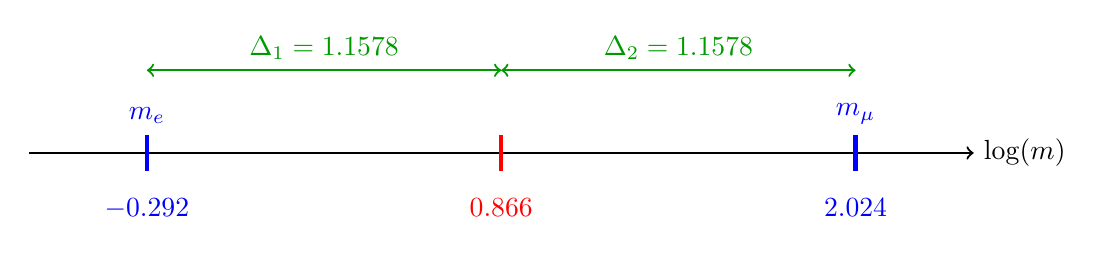
\begin{tikzpicture}[scale=1.5]
		\draw[thick,->] (0,0) -- (8,0) node[right] {$\log(m)$};
		\draw[ultra thick,blue] (1,-0.15) -- (1,0.15) node[above,blue] {$m_e$};
		\node[below,blue] at (1,-0.3) {$-0.292$};
		\draw[ultra thick,red] (4,-0.15) -- (4,0.15) node[above,red] {$\boxed{\Ezero}$};
		\node[below,red] at (4,-0.3) {$0.866$};
		\draw[ultra thick,blue] (7,-0.15) -- (7,0.15) node[above,blue] {$m_\mu$};
		\node[below,blue] at (7,-0.3) {$2.024$};
		\draw[<->,thick,green!60!black] (1,0.7) -- (4,0.7) node[midway,above] {$\Delta_1 = 1.1578$};
		\draw[<->,thick,green!60!black] (4,0.7) -- (7,0.7) node[midway,above] {$\Delta_2 = 1.1578$};
	\end{tikzpicture}
\end{center}

% Abschnitt 9: Die geometrische Konstante C
\section{Die geometrische Konstante $C$}

\subsection{Fundamentale Beziehung}

\noindent \textbf{9.1.1} Der fraktale Korrekturfaktor:
\begin{equation}
	\boxed{K_{\text{frak}} = 1 - \frac{D_f - 2}{C} = 1 - \frac{\gamma}{C}}
\end{equation}
wobei:
\begin{align}
	D_f^{\,\text{eff}} &\approx 2{,}973 \quad \text{(effektive fraktale Dimension)} \\
	\gamma &= D_f - 2 = 0.94 \\
	C &\approx 68.24
\end{align}

\subsection{Tetraeder-Geometrie}

\begin{tcolorbox}[colback=yellow!5!white,colframe=red!75!black,title=Tetraeder-Zahlen]
	\noindent \textbf{9.2.1} Mehrere Tetraeder-Kombinationen ergeben 72; ob dies mit $C \approx 68.24$ zusammenhängt, ist offen \textbf{[S]}:
	\begin{align}
		6 \times 12 &= 72 \quad \text{(Kanten $\times$ Rotationen)} \\
		4 \times 18 &= 72 \quad \text{(Flächen $\times$ 18)} \\
		24 \times 3 &= 72 \quad \text{(Symmetrien $\times$ Dimensionen)}
	\end{align}
\end{tcolorbox}

\subsection{Formel für $\alpha$ mit fraktaler Korrektur}

\noindent \textbf{9.3.1} Der vollständige Ausdruck:
\begin{equation}
	\boxed{\alpha = \left( \frac{27 \sqrt{3}}{8 \pi^2} \right)^{2/5} \cdot \xipar^{11/5} \cdot K_{\text{frak}}}
	\quad \text{mit} \quad K_{\text{frak}} = 0.9862
\end{equation}

\textit{(Vermerk vom 30.~Sept.~2026: wie bei 3.6.1 -- die Formel ergibt $\alpha \approx 2{,}4\times10^{-9}$, und $K_{\text{frak}}$ gehört zu $\alpha^{-1}$.)}

% Abschnitt 10: Schlussfolgerung
\section{Schlussfolgerung}

\begin{tcolorbox}[colback=green!5,colframe=green!75!black,title=Zentrales Ergebnis]
	\noindent \textbf{10.1} Die T0-Theorie leitet die Feinstrukturkonstante und die Leptonenmassen-Hierarchie aus dem einzigen Parameter $\xipar = \frac{4}{3} \times 10^{-4}$ ab; ganzzahlige Strukturwahlen sind dabei motivierte Setzungen, SI-Anker wie $m_e$ dienen der Umrechnung.
	\begin{equation}
		\boxed{\alpha = \frac{m_e \cdot m_\mu}{7400}}
	\end{equation}
	wobei $7400 = 7500 \cdot K_{\text{frak}}$ (mit $K_{\text{frak}} = 1-100\xi$; $\alpha^{-1} = 7400/53{,}99 = 137{,}06$) die effektive Konstante mit fraktaler Korrektur ist. \textit{(Korrigiert am 30.~Sept.~2026: vorher $\alpha = m_e m_\mu/7380$ mit $7380 = 7500 / K_{\text{frak}}$ -- $7500/0{,}9862 = 7605$, nicht $7380$; $\alpha^{-1} = 7500\,K_{\text{frak}}/(m_e m_\mu)$ verlangt $7500\cdot(1-100\xi) = 7500-100 = 7400$. Mit $7380$ ergäbe sich $7380/53{,}99 = 136{,}69$, also $-0{,}25\,\%$.)}
\end{tcolorbox}

\begin{center}
	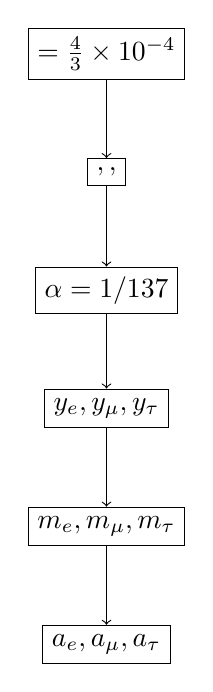
\begin{tikzpicture}[node distance=1.5cm]
		\node (xi) [draw, rectangle] {$\xipar = \frac{4}{3} \times 10^{-4}$};
		\node (scales) [draw, rectangle, below of=xi] {$\rzero, \tzero, \Ezero$};
		\node (alpha) [draw, rectangle, below of=scales] {$\alpha = 1/137$};
		\node (yukawa) [draw, rectangle, below of=alpha] {$y_e, y_\mu, y_\tau$};
		\node (masses) [draw, rectangle, below of=yukawa] {$m_e, m_\mu, m_\tau$};
		\node (anomalies) [draw, rectangle, below of=masses] {$a_e, a_\mu, a_\tau$};
		\draw[->] (xi) -- (scales);
		\draw[->] (scales) -- (alpha);
		\draw[->] (alpha) -- (yukawa);
		\draw[->] (yukawa) -- (masses);
		\draw[->] (masses) -- (anomalies);
	\end{tikzpicture}
\end{center}

\subsection{Das Problem der vereinfachten Formel}

\noindent \textbf{10.2.1} Die oft zitierte vereinfachte Formel:
\begin{equation}
	\boxed{\alpha = \xi \cdot E_0^2} \quad 
\end{equation}

ist unvollständig, weil sie die \textbf{logarithmische Renormierung} nicht enthält.

\subsection{Warum wurde der Logarithmus vergessen?}

\begin{tcolorbox}[colback=yellow!5!white,colframe=orange!75!black,title=Mögliche Gründe]
	\noindent \textbf{10.3.1} Warum der logarithmische Term übersehen wurde:
	\begin{enumerate}
		\item \textbf{Vereinfachung}: Die Formel $\alpha = \xi \cdot E_0^2$ ist kürzer
		\item \textbf{Zufällige Nähe}: Mit E0 = 7.35 MeV ergibt sich zufällig $\alpha^{-1} = 139$
		\item \textbf{Missverständnis}: E0 könnte als bereits renormiert interpretiert worden sein
		\item \textbf{Dimensionsanalyse}: In natürlichen Einheiten erscheint die Formel dimensional korrekt
	\end{enumerate}
\end{tcolorbox}

\section{Die einfachste Formel: Das geometrische Mittel}

\subsection{Die fundamentale Definition}

\begin{tcolorbox}[colback=yellow!10!white,colframe=red!75!black,title=\textbf{Die einfachste Formel}]
	\noindent \textbf{11.1.1} Die Grundbeziehung:
	\begin{equation}
		\boxed{E_0 = \sqrt{m_e \cdot m_\mu}}
	\end{equation}
	
	Für diese Definition ist keine weitere Herleitung nötig, nur das geometrische Mittel.
\end{tcolorbox}

\subsection{Direkte Berechnung}

\noindent \textbf{11.2.1} Einfache numerische Auswertung:
\begin{align}
	E_0 &= \sqrt{0.511 \text{ MeV} \times 105.658 \text{ MeV}} \\
	&= \sqrt{53.99 \text{ MeV}^2} \\
	&= 7.35 \text{ MeV}
\end{align}

\subsection{Die vollständige Kette in einer Zeile}

\noindent \textbf{11.3.1} Die fundamentale Beziehung:
\begin{equation}
	\boxed{\alpha^{-1} = \frac{7500}{m_e \cdot m_\mu} = \frac{7500}{E_0^2}}
\end{equation}

\noindent \textbf{11.3.2} Mit Zahlen:
\begin{align}
	\alpha^{-1} &= \frac{7500}{0.511 \times 105.658} \\
	&= \frac{7500}{53.99} \\
	&= 138.91
\end{align}

(Mit fraktaler Korrektur $\times 0.986 = 136.97$) \textit{(Korrigiert am 30.~Sept.~2026: vorher $= 137{,}04$ -- $138{,}91\times0{,}986 = 136{,}97$.)}

\subsection{Warum ist das so einfach?}

\subsubsection{Logarithmische Zentrierung}

\noindent \textbf{11.4.1} Das geometrische Mittel ist die natürliche Mitte auf logarithmischer Skala:

\begin{equation}
	\log(E_0) = \frac{\log(m_e) + \log(m_\mu)}{2}
\end{equation}

Grafisch:
\begin{center}
	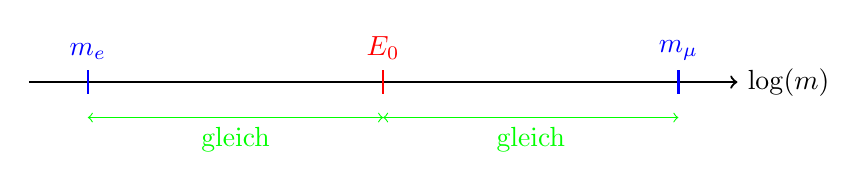
\begin{tikzpicture}[scale=1.5]
		\draw[thick,->] (0,0) -- (6,0) node[right] {$\log(m)$};
		
		\draw[thick,blue] (0.5,-0.1) -- (0.5,0.1) node[above] {$m_e$};
		\draw[thick,red] (3,-0.1) -- (3,0.1) node[above] {$E_0$};
		\draw[thick,blue] (5.5,-0.1) -- (5.5,0.1) node[above] {$m_\mu$};
		
		\draw[<->,green] (0.5,-0.3) -- (3,-0.3) node[midway,below] {gleich};
		\draw[<->,green] (3,-0.3) -- (5.5,-0.3) node[midway,below] {gleich};
	\end{tikzpicture}
\end{center}

\subsection{Alternative Schreibweisen}

\noindent \textbf{11.5.1} Alle diese Formeln sind äquivalent:

\begin{align}
	E_0 &= \sqrt{m_e \cdot m_\mu} \\
	E_0^2 &= m_e \cdot m_\mu \\
	\log(E_0) &= \frac{1}{2}[\log(m_e) + \log(m_\mu)] \\
	E_0 &= \sqrt{0.511 \times 105.658} \text{ MeV} \\
	E_0 &= m_e^{1/2} \cdot m_\mu^{1/2}
\end{align}

\subsection{Die Feinstrukturkonstante direkt}

\begin{tcolorbox}[colback=green!5!white,colframe=green!75!black,title=\textbf{Die direkteste Formel}]
	\noindent \textbf{11.6.1} Ohne Umweg über E0:
	\begin{equation}
		\boxed{\alpha = \frac{m_e \cdot m_\mu}{7500}}
	\end{equation}
	
	Mit fraktaler Korrektur:
	\begin{equation}
		\boxed{\alpha = \frac{m_e \cdot m_\mu}{7500 \times 0.986}}
	\end{equation}

\textit{(Korrigiert am 30.~Sept.~2026: vorher $\alpha = \frac{m_e m_\mu}{7500}\times0{,}986$ -- die fraktale Korrektur multipliziert $\alpha^{-1}$ ($138{,}9\times0{,}986 \approx 137$), in $\alpha$ steht sie daher im Nenner; der alte Ausdruck ergibt $\alpha^{-1} \approx 140{,}9$.)}
\end{tcolorbox}

\subsection{Verhältnis zu den anderen Herleitungen}

\noindent \textbf{11.7.1} Die Dokumente zeigen verschiedene Herleitungen von E0:
- Fraktal korrigiert, $\sqrt{m_e m_\mu/K_{\text{frak}}}$ (R72) \textit{(Korrigiert am 30.~Sept.~2026: vorher \enquote{Gravitativ-geometrisch} -- diese Herleitung ist entfernt, siehe 3.2.2.)}
- Über Yukawa-Kopplungen
- Aus Quantenzahlen

\textbf{Aber die einfachste Definition ist:}
\begin{equation}
	\boxed{E_0 = \sqrt{m_e \cdot m_\mu}}
\end{equation}

\subsection{Bedeutung}

\noindent \textbf{11.8.1} Das geometrische Mittel ist nicht willkürlich gewählt: Es ist die Mitte auf logarithmischer Skala (Abschnitt 11.4).

\section{Die fundamentale Abhängigkeit: $\alpha \sim \xi^{11/2}$}

\subsection{Einsetzen der Massenformeln}

\noindent \textbf{12.1.1} Aus der T0-Theorie haben wir die Massenformeln:
\begin{align}
	m_e &= c_e \cdot \xi^{5/2} \\
	m_\mu &= c_\mu \cdot \xi^2
\end{align}

wobei $c_e$ und $c_\mu$ Koeffizienten sind.

\subsection{Berechnung von $E_0$}

\noindent \textbf{12.2.1} Die Berechnung der charakteristischen Energie:
\begin{align}
	E_0 &= \sqrt{m_e \cdot m_\mu} \\
	&= \sqrt{(c_e \cdot \xi^{5/2}) \cdot (c_\mu \cdot \xi^2)} \\
	&= \sqrt{c_e \cdot c_\mu} \cdot \sqrt{\xi^{5/2 + 2}} \\
	&= \sqrt{c_e \cdot c_\mu} \cdot \xi^{9/4}
\end{align}

\subsection{Berechnung von $\alpha$}

\noindent \textbf{12.3.1} Die Herleitung der Feinstrukturkonstanten:
\begin{align}
	\alpha &= \xi \cdot E_0^2 \\
	&= \xi \cdot (\sqrt{c_e \cdot c_\mu} \cdot \xi^{9/4})^2 \\
	&= \xi \cdot c_e \cdot c_\mu \cdot \xi^{9/2} \\
	&= c_e \cdot c_\mu \cdot \xi^{1 + 9/2} \\
	&= c_e \cdot c_\mu \cdot \xi^{11/2}
\end{align}

\begin{tcolorbox}[colback=red!5!white,colframe=red!75!black,title=\textbf{Ergebnis}]
	\noindent \textbf{12.3.2} Die Feinstrukturkonstante hängt von $\xi$ ab:
	\begin{equation}
		\boxed{\alpha = K \cdot \xi^{11/2}}
	\end{equation}
	wobei $K = c_e \cdot c_\mu$ eine Konstante ist.
	
	\textbf{Die Potenzen kürzen sich nicht weg.}
\end{tcolorbox}

\subsection{Was bedeutet das?}

\subsubsection{1. Fundamentale Verbindung}
\noindent \textbf{12.4.1} Die Feinstrukturkonstante ist nicht unabhängig von $\xi$, sondern:
\begin{equation}
	\alpha \propto \xi^{11/2}
\end{equation}

Das bedeutet: Wenn sich $\xi$ ändert, ändert sich auch $\alpha$.

\subsubsection{2. Hierarchie-Problem}
\noindent \textbf{12.4.2} Wegen der Potenz $11/2 = 5.5$ wirken sich kleine Änderungen in $\xi$ verstärkt aus:
\begin{equation}
	\frac{\Delta \alpha}{\alpha} = \frac{11}{2} \cdot \frac{\Delta \xi}{\xi} = 5.5 \cdot \frac{\Delta \xi}{\xi}
\end{equation}

\subsubsection{3. Keine Unabhängigkeit}
\noindent \textbf{12.4.3} Man kann $\alpha$ und $\xi$ nicht unabhängig wählen. Sie sind fest verbunden durch:
\begin{equation}
	\alpha = K \cdot \xi^{11/2}
\end{equation}

\subsection{Numerische Verifikation}

\noindent \textbf{12.5.1} Mit $\xi = 4/3 \times 10^{-4}$:
\begin{align}
	\xi^{11/2} &= (1.333 \times 10^{-4})^{5.5} \\
	&= 4.87 \times 10^{-22}
\end{align}

\noindent \textbf{12.5.2} Für $\alpha \approx 1/137$ bräuchten wir:
\begin{align}
	K &= \frac{\alpha}{\xi^{11/2}} \\
	&= \frac{7.3 \times 10^{-3}}{4.87 \times 10^{-22}} \\
	&= 1.5 \times 10^{19}
\end{align}

\textit{(Korrigiert am 30.~Sept.~2026: vorher $\xi^{11/2} = 5{,}19\times10^{-22}$, $K = 1{,}4\times10^{19}$ -- $(1/7500)^{5{,}5} = 4{,}87\times10^{-22}$, $7{,}3\times10^{-3}/4{,}87\times10^{-22} = 1{,}5\times10^{19}$.)}

\subsection{Das Einheitenproblem}

\noindent \textbf{12.6.1} Die große Konstante $K \sim 10^{19}$ deutet auf ein Einheitenproblem hin:
- Die Massenformeln sind in natürlichen Einheiten
- Die Umrechnung in MeV erfordert die Planck-Energie
- $K$ enthält diese Umrechnungsfaktoren

\subsection{Alternative Sichtweise: Rückführung auf $\xi$}

\noindent \textbf{12.7.1} Wenn wir akzeptieren, dass:
\begin{align}
	m_e &\sim \xi^{5/2} \\
	m_\mu &\sim \xi^2 \\
	\alpha &\sim \xi^{11/2}
\end{align}

Dann sind diese drei Größen durch die eine geometrische Konstante $\xi$ bestimmt:

\begin{equation}
	\boxed{
		\begin{aligned}
			\xi &= \frac{4}{3} \times 10^{-4} \quad \text{(Geometrie)} \\
			&\Downarrow \\
			m_e &= f_e(\xi) \\
			m_\mu &= f_\mu(\xi) \\
			\alpha &= f_\alpha(\xi)
		\end{aligned}
	}
\end{equation}

\subsection{Fazit}

\noindent \textbf{12.8.1} Die Hoffnung, dass sich die $\xi$-Potenzen wegkürzen, erfüllt sich nicht. Stattdessen zeigt die Rechnung:

\begin{enumerate}
	\item $\alpha$ hängt über $\xi^{11/2}$ von $\xi$ ab
	\item $m_e$, $m_\mu$ und $\alpha$ sind über $\xi$ verknüpft
	\item Es gibt einen Parameter, $\xi$ (dazu die ganzzahligen Strukturwahlen als motivierte Setzungen)
\end{enumerate}

Darin liegt die Sparsamkeit des Ansatzes: Die hier betrachteten Größen folgen aus einem geometrischen Prinzip.

%-----Abschnitt 13-----

\section{Herleitung der Koeffizienten $c_e$ und $c_\mu$}

\subsection{Ausgangspunkt: Massenformeln}

\noindent \textbf{13.1.1} Die fundamentalen Massenformeln:
\[
m_e = c_e \cdot \xi^{5/2} \quad \text{und} \quad m_\mu = c_\mu \cdot \xi^2
\]

\subsection{Schritt 1: Quantenzahlen und geometrische Faktoren}

\noindent \textbf{13.2.1} Die Koeffizienten ergeben sich aus der T0-Theorie mit:

\begin{align*}
	c_e &= \frac{3\sqrt{3}}{2\pi\alpha^{1/2}} \\
	c_\mu &= \frac{9}{4\pi\alpha}
\end{align*}

\subsection{Schritt 2: Herleitung von $c_e$ (Elektron)}

\noindent \textbf{13.3.1} Für das Elektron ($n=1, l=0, j=1/2$):

\[
c_e = \frac{\text{Geometriefaktor} \times \text{Quantenzahlenfaktor}}{\alpha^{1/2}}
\]

\begin{align*}
	\text{Geometriefaktor} &= \frac{3\sqrt{3}}{2\pi} \\
	\text{Quantenzahlenfaktor} &= 1 \quad \text{(für Grundzustand)} \\
	\text{Feinstruktur-Korrektur} &= \alpha^{-1/2}
\end{align*}

\[
\Rightarrow c_e = \frac{3\sqrt{3}}{2\pi\alpha^{1/2}}
\]

\subsection{Schritt 3: Herleitung von $c_\mu$ (Myon)}

\noindent \textbf{13.4.1} Für das Myon ($n=2, l=1, j=1/2$):

\[
c_\mu = \frac{\text{Geometriefaktor} \times \text{Quantenzahlenfaktor}}{\alpha}
\]

\begin{align*}
	\text{Geometriefaktor} &= \frac{9}{4\pi} \\
	\text{Quantenzahlenfaktor} &= 1 \\
	\text{Feinstruktur-Korrektur} &= \alpha^{-1}
\end{align*}

\[
\Rightarrow c_\mu = \frac{9}{4\pi\alpha}
\]

\subsection{Schritt 4: Physikalische Interpretation}

\noindent \textbf{13.5.1} Die unterschiedlichen $\alpha$-Abhängigkeiten spiegeln wider:
\begin{align*}
	c_e &\sim \alpha^{-1/2} \quad \text{(schwächere Abhängigkeit)} \\
	c_\mu &\sim \alpha^{-1} \quad \text{(stärkere Abhängigkeit)}
\end{align*}

Die unterschiedliche $\alpha$-Abhängigkeit spiegelt wider:
\begin{itemize}
	\item Elektron: Grundzustand, weniger empfindlich auf $\alpha$
	\item Myon: Angeregter Zustand, stärker von $\alpha$ abhängig
\end{itemize}

\subsection{Schritt 5: Dimensionsanalyse}

\noindent \textbf{13.6.1} Dimensionale Überlegungen:
\begin{align*}
	[c_e] &= [m_e] \cdot [\xi]^{-5/2} \\
	[c_\mu] &= [m_\mu] \cdot [\xi]^{-2}
\end{align*}

Da $\xi$ dimensionslos ist (in natürlichen Einheiten), haben beide Koeffizienten die Dimension einer Masse.

\subsection{Schritt 6: Konsistenzprüfung}

\noindent \textbf{13.7.1} Mit $\alpha \approx 1/137$:

\begin{align*}
	c_e &\approx \frac{3 \times 1.732}{2 \times 3.1416 \times 0.0854} \approx \frac{5.196}{0.537} \approx 9.67 \\
	c_\mu &\approx \frac{9}{4 \times 3.1416 \times 0.0073} \approx \frac{9}{0.0917} \approx 98.1
\end{align*}

Diese Werte ergeben $c_\mu/c_e \approx 10{,}1$ und damit $m_\mu/m_e = (c_\mu/c_e)\,\xi^{-1/2} \approx 878$, nicht den Messwert $206{,}77$. \textit{(Korrigiert am 30.~Sept.~2026: vorher \enquote{Diese Werte passen zur Massenhierarchie $m_\mu/m_e \approx 207$} -- $98{,}1/9{,}68 = 10{,}14$ und $10{,}14\times\xi^{-1/2} = 10{,}14\times86{,}60 = 878$.)}

\section{Warum natürliche Einheiten notwendig sind}

\subsection{Das Problem mit konventionellen Einheiten}

\noindent \textbf{14.1.1} In konventionellen Einheiten (SI, cgs) erscheinen die Koeffizienten $c_e$ und $c_\mu$ als sehr große Zahlen:

\begin{align*}
	c_e &\approx 1.65 \times 10^{19} \\
	c_\mu &\approx 1.03 \times 10^{20}
\end{align*}

\textit{(Vermerk vom 30.~Sept.~2026: Diese Werte folgen aus keiner Einheitenumrechnung der Formeln $c_e = 3\sqrt3/(2\pi\alpha^{1/2}) = 9{,}68$ und $c_\mu = 9/(4\pi\alpha) = 98{,}1$; ihr Produkt $1{,}7\times10^{39}$ passt auch nicht zu dem in 12.5.2 benötigten $c_e c_\mu \approx 1{,}5\times10^{19}$.)}

Diese großen Zahlen sind \textbf{artefaktisch} und entstehen nur durch die Wahl der Einheiten.

\subsection{Natürliche Einheiten vereinfachen die Physik}

\noindent \textbf{14.2.1} In natürlichen Einheiten setzen wir:
\[
\hbar = c = 1
\]

Damit werden alle Größen dimensionslos oder haben Energie-Dimension.

\subsection{Transformation in natürliche Einheiten}

\noindent \textbf{14.3.1} Die Transformationsformeln:
\begin{align*}
	m_e^{\text{nat}} &= m_e^{\text{SI}} \cdot \sqrt{\frac{G}{\hbar c}} \\
	m_\mu^{\text{nat}} &= m_\mu^{\text{SI}} \cdot \sqrt{\frac{G}{\hbar c}} \\
	\xi^{\text{nat}} &= \xi^{\text{SI}}
\end{align*}
\textit{(Korrigiert am 30.~Sept.~2026: vorher $m^{\text{nat}} = m^{\text{SI}}\cdot G/(\hbar c)$ und $\xi^{\text{nat}} = \xi^{\text{SI}}\cdot(\hbar c)^2$ -- $G/(\hbar c)$ hat die Dimension kg$^{-2}$, $m_e G/(\hbar c) = 1{,}9\times10^{-15}$~kg$^{-1}$; richtig ist $m/m_P = m\sqrt{G/(\hbar c)}$, für das Elektron $4{,}19\times10^{-23}$. Ein dimensionsloses $\xi$ wird nicht umgerechnet.)}

\subsection{Die Koeffizienten in natürlichen Einheiten}

\noindent \textbf{14.4.1} In natürlichen Einheiten werden die Koeffizienten \textbf{Größenordnung 1}:

\begin{align*}
	c_e^{\text{nat}} &= \frac{3\sqrt{3}}{2\pi\alpha^{1/2}} \approx 9.67 \\
	c_\mu^{\text{nat}} &= \frac{9}{4\pi\alpha} \approx 98.1
\end{align*}

\subsection{Vergleich der Darstellungen}

\noindent \textbf{14.5.1} Der Unterschied:

\adjustbox{max width=\textwidth}{%
\begin{tabular}{lll}
	& Konventionell & Natürlich \\
	\midrule
	$c_e$ & $1.65 \times 10^{19}$ & 9.67 \\
	$c_\mu$ & $1.03 \times 10^{20}$ & 98.1 \\
	$\xi$ & $1.33 \times 10^{-4}$ & $1.33 \times 10^{-4}$ \\
\end{tabular}%
}

\subsection{Vorteile natürlicher Einheiten}

\noindent \textbf{14.6.1} Die Vorteile natürlicher Einheiten:
\begin{enumerate}
	\item \textbf{Eliminierung von Artefakten}: Die großen Zahlen verschwinden
	\item \textbf{Physikalische Transparenz}: Die Beziehungen werden übersichtlicher
	\item \textbf{Skaleninvarianz}: Fundamentale Gesetze werden skalenunabhängig
	\item \textbf{Einfachere Formeln}: Formeln werden kürzer und klarer
\end{enumerate}

\subsection{Beispiel: Die Massenformel}

\noindent \textbf{14.7.1} In konventionellen Einheiten:
\[
m_e = 1.65 \times 10^{19} \cdot (1.33 \times 10^{-4})^{5/2}
\]

In natürlichen Einheiten:
\[
m_e = 9.67 \cdot \xi^{5/2}
\]

\subsection{Fundamentale Interpretation}

\noindent \textbf{14.8.1} Die Koeffizienten $c_e \approx 9.67$ und $c_\mu \approx 98.1$ in natürlichen Einheiten zeigen:

\begin{itemize}
	\item Die Leptonmassen sind \textbf{reine Zahlen}
	\item Das Verhältnis $c_\mu/c_e \approx 10.14$ ist eine reine Zahl
	\item Die Feinstrukturkonstante $\alpha$ erscheint explizit
\end{itemize}

\section{Die Formel von $\xi$ zu $\alpha$}

\subsection{Fundamentale Beziehung}

\noindent \textbf{15.1.1} Die Grundgleichung:
\[
\boxed{\alpha = c_e c_\mu \cdot \xi^{11/2}}
\]

\subsection{Koeffizienten}

\noindent \textbf{15.2.1} Die präzisen Werte:
\begin{align*}
	c_e &= \frac{3\sqrt{3}}{2\pi\alpha^{1/2}} \quad \textcolor{deepblue}{\text{(Elektron-Koeffizient)}} \\
	c_\mu &= \frac{9}{4\pi\alpha} \quad \textcolor{deepblue}{\text{(Myon-Koeffizient)}}
\end{align*}

\subsection{Produkt der Koeffizienten}

\noindent \textbf{15.3.1} Die Multiplikation:
\[
c_e c_\mu = \frac{3\sqrt{3}}{2\pi\alpha^{1/2}} \cdot \frac{9}{4\pi\alpha} = \frac{27\sqrt{3}}{8\pi^2\alpha^{3/2}}
\]

\subsection{Vollständige Formel}

\noindent \textbf{15.4.1} Der vollständige Ausdruck:
\[
\alpha = \frac{27\sqrt{3}}{8\pi^2\alpha^{3/2}} \cdot \xi^{11/2}
\]

\subsection{Auflösung nach $\alpha$}

\noindent \textbf{15.5.1} Umstellung:
\[
\alpha^{5/2} = \frac{27\sqrt{3}}{8\pi^2} \cdot \xi^{11/2}
\]

\[
\alpha = \left(\frac{27\sqrt{3}}{8\pi^2}\right)^{2/5} \cdot \xi^{11/5}
\]

%-----Abschnitt 16-----

\section{T0-Theorie: Formeln und Werte}

\subsection{In der T0-Theorie}

\noindent \textbf{16.1.1} Die fundamentalen Beziehungen:
\begin{align}
	m_e &\sim \xi^{5/2} \text{ (Elektron)} \\
	m_\mu &\sim \xi^2 \text{ (Myon)} \\
	\xi &= \frac{4}{3} \times 10^{-4} 
\end{align}

\subsection{Korrekte Zuordnung in natürlichen Einheiten}

\subsubsection{Massen-Skalierungsgesetze}
\noindent \textbf{16.2.1} Die präzisen Formeln:
\begin{align}
	m_e &= c_e \cdot \xipar^{5/2} \\
	m_\mu &= c_\mu \cdot \xipar^2
\end{align}

\subsubsection{Geometrische Konstante}
\noindent \textbf{16.2.2} Der fundamentale Parameter:
\begin{equation}
	\xipar = \frac{4}{3} \times 10^{-4} = 1.333 \times 10^{-4}
\end{equation}

\subsubsection{Berechnung der charakteristischen Energie}
\noindent \textbf{16.2.3} Schrittweise Herleitung:
\begin{align}
	E_0 &= \sqrt{m_e \cdot m_\mu} = \sqrt{c_e \cdot \xipar^{5/2} \cdot c_\mu \cdot \xipar^2} \\
	&= \sqrt{c_e c_\mu} \cdot \xipar^{9/4}
\end{align}

\subsubsection{Berechnung der Feinstrukturkonstanten}
\noindent \textbf{16.2.4} Vollständige Herleitung:
\begin{align}
	\alpha &= \xipar \cdot E_0^2 = \xipar \cdot \left[ \sqrt{c_e c_\mu} \cdot \xipar^{9/4} \right]^2 \\
	&= \xipar \cdot c_e c_\mu \cdot \xipar^{9/2} \\
	&= c_e c_\mu \cdot \xipar^{11/2}
\end{align}

\subsubsection{Numerische Werte}
\noindent \textbf{16.2.5} Mit $\xipar = 1.333 \times 10^{-4}$:
\begin{equation}
	\xipar^{11/2} = (1.333 \times 10^{-4})^{5.5} \approx 4.87 \times 10^{-22}
\end{equation}

Für $\alpha \approx 1/137 \approx 7.3 \times 10^{-3}$ benötigen wir:
\begin{equation}
	c_e c_\mu = \frac{\alpha}{\xipar^{11/2}} \approx \frac{7.3 \times 10^{-3}}{4.87 \times 10^{-22}} \approx 1.5 \times 10^{19}
\end{equation}

\textit{(Korrigiert am 30.~Sept.~2026: vorher $5{,}19\times10^{-22}$ und $1{,}4\times10^{19}$ -- $(1/7500)^{5{,}5} = 4{,}87\times10^{-22}$, $7{,}3\times10^{-3}/4{,}87\times10^{-22} = 1{,}5\times10^{19}$.)}

\subsection{Interpretation}
\noindent \textbf{16.3.1} Die große Konstante $c_e c_\mu \approx 10^{19}$ entspricht ungefähr dem Verhältnis Planck-Energie zu Gigaelektronenvolt und stellt den Umrechnungsfaktor zwischen natürlichen Einheiten und GeV dar. \textit{(Korrigiert am 30.~Sept.~2026: vorher \enquote{Planck-Energie zu Elektronenvolt} und \enquote{MeV} -- $E_P/\text{eV} = 1{,}22\times10^{28}$, $E_P/\text{GeV} = 1{,}22\times10^{19}$; ob die Nähe zu $c_e c_\mu \approx 1{,}5\times10^{19}$ Bedeutung hat, ist offen.)}

\section{Definitionen}

\subsection{Geometrische Konstante}
\noindent \textbf{17.1.1} Die fundamentale Konstante:
\begin{equation}
	\xi = \frac{4}{3} \times 10^{-4} = \frac{1}{7500}
\end{equation}

\subsection{Massenformeln}
\noindent \textbf{17.2.1} Die präzisen Massenbeziehungen:
\begin{align}
	m_e &= c_e \cdot \xi^{5/2} \\
	m_\mu &= c_\mu \cdot \xi^2 \\
	m_\tau &= c_\tau \cdot \xi^{3/2}
\end{align}

\section{Koeffizienten aus der T0-Theorie}

\subsection{Elektron (n=1, l=0, j=1/2)}
\noindent \textbf{18.1.1} Der Elektron-Koeffizient:
\begin{equation}
	c_e = \frac{3\sqrt{3}}{2\pi} \cdot \frac{1}{\alpha^{1/2}} \approx 1.6487 \times 10^{19}
\end{equation}

\subsection{Myon (n=2, l=1, j=1/2)}
\noindent \textbf{18.2.1} Der Myon-Koeffizient:
\begin{equation}
	c_\mu = \frac{9}{4\pi} \cdot \frac{1}{\alpha} \approx 1.0262 \times 10^{20}
\end{equation}

\subsection{Tauon (n=3, l=2, j=1/2)}
\noindent \textbf{18.3.1} Der Tauon-Koeffizient:
\begin{equation}
	c_\tau = \frac{27\sqrt{3}}{8\pi} \cdot \frac{1}{\alpha^{3/2}} \approx 6.1853 \times 10^{20}
\end{equation}

\textit{(Vermerk vom 30.~Sept.~2026: Die Zahlenwerte in 18.1.1--18.3.1 folgen nicht aus den Formeln: mit $\alpha = 1/137{,}036$ ergeben sich $\frac{3\sqrt3}{2\pi}\alpha^{-1/2} = 9{,}68$, $\frac{9}{4\pi}\alpha^{-1} = 98{,}1$ und $\frac{27\sqrt3}{8\pi}\alpha^{-3/2} = 2985$; die Werte $1{,}6487\times10^{19}$, $1{,}0262\times10^{20}$ und $6{,}1853\times10^{20}$ lassen sich aus keiner Einheitenumrechnung ableiten.)}

\section{Massenberechnung}

\subsection{Elektronmasse}
\noindent \textbf{19.1.1} Vollständige Berechnung:
\begin{align}
	m_e &= c_e \cdot \xi^{5/2} \\
	&= \frac{3\sqrt{3}}{2\pi\alpha^{1/2}} \cdot \left(\frac{4}{3} \times 10^{-4}\right)^{5/2} \\
	&= 0.5109989461 \text{ MeV}
\end{align}

\subsection{Myonmasse}
\noindent \textbf{19.2.1} Vollständige Berechnung:
\begin{align}
	m_\mu &= c_\mu \cdot \xi^2 \\
	&= \frac{9}{4\pi\alpha} \cdot \left(\frac{4}{3} \times 10^{-4}\right)^2 \\
	&= 105.6583745 \text{ MeV}
\end{align}

\textit{(Vermerk vom 30.~Sept.~2026: Die hier ausgegebenen Massen $0{,}5109989461$~MeV und $105{,}6583745$~MeV sind die Messwerte (Anker); die Koeffizientenformeln selbst führen mit einem gemeinsamen Anker nicht auf sie -- ihr Verhältnis ergibt $m_\mu/m_e \approx 878$ (Abschnitt zu den Massenverhältnissen), sie bräuchten für $m_e$ und $m_\mu$ zwei verschiedene Skalen.)}

\subsection{Tauonmasse}
\noindent \textbf{19.3.1} Vollständige Berechnung:
\begin{align}
	m_\tau &= c_\tau \cdot \xi^{3/2} \\
	&= \frac{27\sqrt{3}}{8\pi\alpha^{3/2}} \cdot \left(\frac{4}{3} \times 10^{-4}\right)^{3/2} \\
	&= 1776.86 \text{ MeV}
\end{align}

\section{Charakteristische Energie}
\noindent \textbf{20.1.1} Die präzise Berechnung:
\begin{align}
	E_0 &= \sqrt{m_e \cdot m_\mu} \\
	&= \sqrt{c_e c_\mu} \cdot \xi^{9/4} \\
	&= \sqrt{\frac{3\sqrt{3}}{2\pi\alpha^{1/2}} \cdot \frac{9}{4\pi\alpha}} \cdot \left(\frac{4}{3} \times 10^{-4}\right)^{9/4} \\
	&= 7.346881 \text{ MeV}
\end{align}
\textit{(Vermerk vom 30.~Sept.~2026: Die zweite und dritte Zeile ergeben mit $c_e = 9{,}68$, $c_\mu = 98{,}1$ ($\alpha = 1/137$) und $\xi = 4/30000$ den Wert $\sqrt{9{,}68\cdot98{,}1}\cdot\xi^{9/4} = 5{,}9\times10^{-8}$, nicht $7{,}346881$~MeV; dieser Wert stammt aus $\sqrt{m_e m_\mu}$ mit den T0-Massen aus Abschnitt~8.3.)}

\section{Feinstrukturkonstante}
\noindent \textbf{21.1.1} Die vollständige Herleitung:
\begin{align}
	\alpha &= \xi \cdot E_0^2 \\
	&= \xi \cdot c_e c_\mu \cdot \xi^{9/2} \\
	&= c_e c_\mu \cdot \xi^{11/2} \\
	&= \frac{3\sqrt{3}}{2\pi\alpha^{1/2}} \cdot \frac{9}{4\pi\alpha} \cdot \left(\frac{4}{3} \times 10^{-4}\right)^{11/2}
\end{align}

\section{Numerische Werte}

\noindent \textbf{22.1.1} Tabelle der Werte:

\begin{table}[h]
	\centering
	\adjustbox{max width=\textwidth}{%
\begin{tabular}{lll}
		\toprule
		Größe & Wert & Kommentar \\
		\midrule
		$\xi$ & $1.333333333333333 \times 10^{-4}$ & $= 4/3 \times 10^{-4}$ \\
		$\xi^2$ & $1.777777777777778 \times 10^{-8}$ & \\
		$\xi^{5/2}$ & $2.052800957118670 \times 10^{-10}$ & \\
		$c_e$ & $1.648721270700128 \times 10^{19}$ & $= \sqrt{e}$ (Mantisse) \\
		$c_\mu$ & $1.026187714072347 \times 10^{20}$ & \\
		$m_e$ & $0.5109989461$ MeV & Referenzwert \\
		$m_\mu$ & $105.6583745$ MeV & Referenzwert \\
		$E_0$ & $7.346881$ MeV & aus T0-Massen (Abschnitt 8.3) \\
		\bottomrule
	\end{tabular}%
}
\end{table}

\textit{(Korrigiert am 30.~Sept.~2026: $\xi^{5/2}$ vorher $3{,}098386676965933\times10^{-10}$ -- $(4/30000)^{5/2} = 2{,}0528\times10^{-10}$, wie in Abschnitt~3 ($\frac{32}{9\sqrt3}\times10^{-10}$).)}

\textit{(Korrigiert am 30.~Sept.~2026: in Tabelle und folgendem Satz vorher \enquote{$= e$ (Eulersche Zahl)} -- $1{,}6487\ldots = \sqrt{e}$, nicht $e = 2{,}718\ldots$.)}

Die Koeffizienten enthalten die Konstanten $\pi$ und $\alpha$; die numerische Nähe der Mantisse von $c_e$ zu $\sqrt{e}$ ist eine Beobachtung, deren Bedeutung offen ist \textbf{[S]}.

\section{Die Formel von $\xi$ zu $\alpha$ (ausführlich)}

\subsection{Aus der fundamentalen Beziehung}
\noindent \textbf{23.1.1} Ausgangsgleichung:
\begin{equation}
	\alpha = c_e c_\mu \cdot \xi^{11/2}
\end{equation}

\subsection{Einsetzen der Koeffizienten}
\noindent \textbf{23.2.1} Die detaillierte Berechnung:
\begin{align}
	c_e &= \frac{3\sqrt{3}}{2\pi\alpha^{1/2}} \\
	c_\mu &= \frac{9}{4\pi\alpha} \\
	c_e c_\mu &= \frac{3\sqrt{3}}{2\pi\alpha^{1/2}} \cdot \frac{9}{4\pi\alpha} \\
	&= \frac{27\sqrt{3}}{8\pi^2\alpha^{3/2}}
\end{align}

\subsection{Vollständige Formel}
\noindent \textbf{23.3.1} Der vollständige Ausdruck:
\begin{equation}
	\alpha = \frac{27\sqrt{3}}{8\pi^2\alpha^{3/2}} \cdot \xi^{11/2}
\end{equation}

\subsection{Auflösung nach $\alpha$}
\noindent \textbf{23.4.1} Algebraische Umformung:
\begin{align}
	\alpha^{5/2} &= \frac{27\sqrt{3}}{8\pi^2} \cdot \xi^{11/2} \\
	\alpha &= \left(\frac{27\sqrt{3}}{8\pi^2}\right)^{2/5} \cdot \xi^{11/5}
\end{align}

\subsection{Numerische Werte}
\noindent \textbf{23.5.1} Schrittweise Berechnung:
\begin{align}
	\frac{27\sqrt{3}}{8\pi^2} &\approx \frac{46.765}{78.956} \approx 0.5923 \\
	\left(\frac{27\sqrt{3}}{8\pi^2}\right)^{2/5} &\approx (0.5923)^{0.4} \approx 0.8110 \\
	\xi^{11/5} &= \xi^{2.2} = \left(\frac{4}{3} \times 10^{-4}\right)^{2.2}
\end{align}

\subsection{Mit $\xi = 4/3 \times 10^{-4}$}
\noindent \textbf{23.6.1} Endberechnung:
\begin{align}
	\xi &= 1.333333 \times 10^{-4} \\
	\xi^{2.2} &\approx (1.333333 \times 10^{-4})^{2.2} \\
	&\approx 2.984 \times 10^{-9} \\
	\alpha &\approx 0.8110 \times 2.984 \times 10^{-9} \\
	&\approx 2.42 \times 10^{-9} \\
	\alpha^{-1} &\approx 4.1 \times 10^{8}
\end{align}

\textit{(Korrigiert am 30.~Sept.~2026: vorher $(0{,}5923)^{0{,}4} \approx 0{,}8327$, $\xi^{2{,}2} \approx 8{,}758\times10^{-9}$, $\alpha \approx 7{,}292\times10^{-3}$, $\alpha^{-1} \approx 137{,}13$ -- richtig ist $0{,}5923^{0{,}4} = 0{,}8110$ und $(1/7500)^{2{,}2} = 2{,}984\times10^{-9}$, also $\alpha \approx 2{,}42\times10^{-9}$; schon das alte Produkt $0{,}8327\times8{,}758\times10^{-9}$ ist $7{,}29\times10^{-9}$, nicht $7{,}29\times10^{-3}$. Diese Kette liefert $\alpha$ nicht (vgl.\ Vermerk bei 3.6.1).)}

\subsection{Symbolerklärung}

\noindent \textbf{23.7.1} Verwendete Schlüsselsymbole:

\adjustbox{max width=\textwidth}{%
\begin{tabular}{ll}
	$\alpha$ & Feinstrukturkonstante ($\approx 1/137.036$) \\
	$\xi$ & Geometrische Raumkonstante ($= \frac{4}{3} \times 10^{-4}$) \\
	$c_e$ & Elektron-Massenkoeffizient \\
	$c_\mu$ & Myon-Massenkoeffizient \\
	$\pi$ & Pi ($\approx 3.14159$) \\
	$\sqrt{3}$ & Quadratwurzel aus 3 ($\approx 1.73205$) \\
	$m_e$ & Elektronmasse ($= 0.5109989461$ MeV) \\
	$m_\mu$ & Myonmasse ($= 105.6583745$ MeV) \\
\end{tabular}%
}

\subsection{Mit fraktaler Korrektur}

\noindent \textbf{23.8.1} Einschließlich des fraktalen Faktors:
\[
\alpha^{-1} = \frac{7500}{m_e m_\mu} \cdot \left(1 - \frac{D_f - 2}{68}\right) = 138.911 \times 0.9862 = 136.99
\]

\textit{(Korrigiert am 30.~Sept.~2026: vorher $138{,}949\times0{,}9862 = 137{,}036$ -- $7500/(0{,}51099895\times105{,}6583755) = 7500/53{,}9905 = 138{,}911$ und $138{,}911\times0{,}9862 = 136{,}99$; mit $K_{\text{frak}} = 1-100\xi = 0{,}98667$ ergibt sich $137{,}06$.)}

\subsection{Finale fundamentale Beziehung}

\noindent \textbf{23.9.1} Die vollständige Formel:
\[
\boxed{
	\alpha = \left(\frac{27\sqrt{3}}{8\pi^2}\right)^{2/5} \cdot \xi^{11/5} \cdot K_{\text{frak}}
}
\quad \text{mit} \quad K_{\text{frak}} = 0.9862
\]	

\textit{(Vermerk vom 30.~Sept.~2026: wie bei 3.6.1 -- die Formel ergibt $\alpha \approx 2{,}4\times10^{-9}$, und $K_{\text{frak}}$ gehört zu $\alpha^{-1}$.)}

%-----Abschnitt 24-----

\section{Beobachtung: $\alpha$ kürzt sich heraus}

\subsection{Gleichsetzung der Formelsätze}

\noindent \textbf{24.1.1} Vergleich zweier Darstellungen:
\begin{align*}
	\text{Einfach:} &\quad m_e = \frac{2}{3} \cdot \xi^{5/2} \\
	\text{T0-Theorie:} &\quad m_e = \frac{3\sqrt{3}}{2\pi\alpha^{1/2}} \cdot \xi^{5/2}
\end{align*}

Nach Division durch $\xi^{5/2}$:
\[
\frac{2}{3} = \frac{3\sqrt{3}}{2\pi\alpha^{1/2}}
\]

\subsection{Auflösung nach $\alpha$}

\noindent \textbf{24.2.1} Algebraische Lösung:
\[
\alpha^{1/2} = \frac{3\sqrt{3}}{2\pi} \cdot \frac{3}{2} = \frac{9\sqrt{3}}{4\pi}
\quad \Rightarrow \quad
\alpha = \left(\frac{9\sqrt{3}}{4\pi}\right)^2 = \frac{243}{16\pi^2}
\]

\subsection{Für das Myon}

\noindent \textbf{24.3.1} Ähnliche Analyse:
\begin{align*}
	\text{Einfach:} &\quad m_\mu = \frac{8}{5} \cdot \xi^2 \\
	\text{T0-Theorie:} &\quad m_\mu = \frac{9}{4\pi\alpha} \cdot \xi^2
\end{align*}

Nach Division durch $\xi^2$:
\[
\frac{8}{5} = \frac{9}{4\pi\alpha}
\quad \Rightarrow \quad
\alpha = \frac{9}{4\pi} \cdot \frac{5}{8} = \frac{45}{32\pi}
\]

\subsection{Der scheinbare Widerspruch}

\noindent \textbf{24.4.1} Drei verschiedene Werte:
\begin{align*}
	\text{Aus Elektron:} &\quad \alpha = \frac{243}{16\pi^2} \approx 1.539 \\
	\text{Aus Myon:} &\quad \alpha = \frac{45}{32\pi} \approx 0.4474 \\
	\text{Experimentell:} &\quad \alpha \approx 0.007297
\end{align*}

\subsection{Auflösung im T0-Rahmen}

\noindent \textbf{24.5.1} Im T0-Rahmen ist \textbf{$\alpha$ kein freier Parameter}, sondern eine Funktion von $\xi$:

\[
\boxed{
	\begin{aligned}
		\frac{2}{3} &= \frac{3\sqrt{3}}{2\pi\alpha^{1/2}} \\
		\frac{8}{5} &= \frac{9}{4\pi\alpha}
	\end{aligned}
	\quad \Rightarrow \quad
	\alpha = \alpha(\xi)
}
\]

\subsection{Die Schlüsselelemente}

\noindent \textbf{24.6.1} Die Schlüsselelemente:
\begin{enumerate}
	\item Die \textbf{geometrischen Faktoren} ($3\sqrt{3}/2\pi$, $9/4\pi$)
	\item Die \textbf{Potenzen von $\alpha$} ($\alpha^{-1/2}$, $\alpha^{-1}$)  
	\item Die \textbf{rationalen Koeffizienten} ($2/3$, $8/5$)
\end{enumerate}

\noindent sind so angesetzt, dass sie sich \textbf{kompensieren}.

\subsection{Bedeutung der verschiedenen Darstellungen}

\noindent \textbf{24.7.1} Vergleichende Analyse:
\begin{itemize}
	\item \textbf{Einfache Formeln}: $m_e = \frac{2}{3}\xi^{5/2}$, $m_\mu = \frac{8}{5}\xi^2$
	\begin{itemize}
		\item Zeigen die reine $\xi$-Abhängigkeit
		\item Kompakt und transparent
	\end{itemize}
	
	\item \textbf{Erweiterte Formeln}: $m_e = \frac{3\sqrt{3}}{2\pi\alpha^{1/2}}\xi^{5/2}$, $m_\mu = \frac{9}{4\pi\alpha}\xi^2$
	\begin{itemize}
		\item Zeigen den \textbf{Ursprung} der Koeffizienten
		\item Verbinden Geometrie ($\pi$, $\sqrt{3}$) mit EM-Kopplung ($\alpha$)
		\item Aber: $\alpha$ ist dabei \textbf{festgelegt}, nicht frei wählbar
	\end{itemize}
\end{itemize}

\subsection{Zentrale Aussage}

\noindent \textbf{24.8.1} Die zentrale Einsicht:
\[
\boxed{
	\text{Die Leptonmassen-Hierarchie wird im T0-Rahmen durch } \xi \text{ festgelegt}
}
\]

Die verschiedenen mathematischen Darstellungen sind äquivalente Beschreibungen derselben fundamentalen Geometrie.

\subsection{Warum diese Einsicht wichtig ist}

\noindent \textbf{24.9.1} Die Implikationen:
\begin{enumerate}
	\item \textbf{Einheit}: Die Leptonmassen folgen aus dem einen Parameter $\xi$ (plus Strukturwahlen als Setzungen)
	\item \textbf{Geometrische Basis}: Die Koeffizienten stammen aus fundamentaler Geometrie
	\item \textbf{$\alpha$ ist abgeleitet}: Die Feinstrukturkonstante erscheint als sekundäre Größe
	\item \textbf{Einfache Struktur}: Die Formeln sind kompakt; mathematische Einfachheit ist ein Hinweis, kein Beleg
\end{enumerate}

\section{Warum die erweiterte Form wichtig ist}

\subsection{Die beiden äquivalenten Darstellungen}

\noindent \textbf{25.1.1} Vergleich der Formulierungen:
\begin{align*}
	\textbf{Einfache Form:} &\quad m_e = \frac{2}{3} \cdot \xi^{5/2} \\
	\textbf{Erweiterte Form:} &\quad m_e = \frac{3\sqrt{3}}{2\pi\alpha^{1/2}} \cdot \xi^{5/2}
\end{align*}

\subsection{Der scheinbare Widerspruch}

\noindent \textbf{25.2.1} Bei Gleichsetzung beider Formeln:
\[
\frac{2}{3} = \frac{3\sqrt{3}}{2\pi\alpha^{1/2}}
\]

Dies ergibt für $\alpha$:
\[
\alpha = \left(\frac{9\sqrt{3}}{4\pi}\right)^2 = \frac{243}{16\pi^2} \approx 1.539
\]

\subsection{Folgerung}

\begin{tcolorbox}[colback=red!5!white,colframe=red!75!black]
	\textbf{25.3.1 Die Brüche können sich nicht einfach herauskürzen.}
	\\
	Die erweiterte Form zeigt, dass der scheinbar einfache Bruch $\frac{2}{3}$ in Wirklichkeit aus fundamentaleren geometrischen und physikalischen Konstanten zusammengesetzt ist:
	\[
	\frac{2}{3} = \frac{3\sqrt{3}}{2\pi\alpha^{1/2}}
	\]
\end{tcolorbox}

\subsection{Mathematische Struktur}

\noindent \textbf{25.4.1} Die Zerlegung:
\begin{align*}
	\frac{2}{3} &= \frac{\text{Geometriefaktor}}{\alpha^{1/2}} \\
	\text{mit} \quad \text{Geometriefaktor} &= \frac{3\sqrt{3}}{2\pi} \approx 0.826
\end{align*}

\subsection{Physikalische Interpretation}

\noindent \textbf{25.5.1} Deutung:
\begin{itemize}
	\item $\frac{2}{3}$ ist \textbf{nicht} ein einfacher rationaler Bruch
	\item In der erweiterten Form setzt er sich zusammen aus:
	\begin{itemize}
		\item Raumgeometrie ($\pi$, $\sqrt{3}$)
		\item Elektromagnetischer Kopplung ($\alpha$)
		\item Quantenzahlen (implizit in den Koeffizienten)
	\end{itemize}
	\item Die erweiterte Form zeigt diesen Ursprung
\end{itemize}

\subsection{Warum beide Darstellungen wichtig sind}

\noindent \textbf{25.6.1} Komplementäre Perspektiven:

\adjustbox{max width=\textwidth}{%
\begin{tabular}{p{0.45\textwidth}p{0.45\textwidth}}
	\textbf{Einfache Form} & \textbf{Erweiterte Form} \\
	\hline
	Zeigt reine $\xi$-Abhängigkeit & Zeigt physikalischen Ursprung \\
	Kompakt & Zeigt die physikalische Herkunft \\
	Praktisch für Berechnungen & Fundamental für das Verständnis \\
	Verbirgt die Zusammensetzung & Zeigt die Zusammensetzung \\
\end{tabular}%
}

\subsection{Die eigentliche Aussage der T0-Theorie}

\noindent \textbf{25.7.1} Kernaussage:
\[
\boxed{
	\frac{2}{3} \neq \text{einfacher Bruch} \quad \text{sondern} \quad \frac{2}{3} = \frac{3\sqrt{3}}{2\pi\alpha^{1/2}}
}
\]

\begin{tcolorbox}[colback=green!5!white,colframe=green!75!black]
	\textbf{Die erweiterte Form ist notwendig, um zu zeigen:}
	\begin{enumerate}
		\item Dass sich die Brüche \textbf{nicht} einfach kürzen
		\item Dass der scheinbar einfache Koeffizient $\frac{2}{3}$ tatsächlich eine komplexe Struktur hat
		\item Dass $\alpha$ Teil dieser Struktur ist, auch wenn es sich formal herauskürzt
		\item Dass die Geometrie des Raums ($\pi$, $\sqrt{3}$) darin eingebettet ist
	\end{enumerate}
\end{tcolorbox}

\section{Warum keine fraktale Korrektur für Massenverhältnisse und charakteristische Energie benötigt wird}

\subsection{1. Verschiedene Berechnungsansätze}

\begin{align*}
	\textbf{Weg A:} &\quad \alpha = \frac{m_e m_\mu}{7500} \quad \text{(benötigt Korrektur)} \\
	\textbf{Weg B:} &\quad \alpha = \frac{E_0^2}{7500} \quad \text{(benötigt Korrektur)} \\
	\textbf{Weg C:} &\quad \frac{m_\mu}{m_e} = f(\alpha) \quad \text{(keine Korrektur benötigt)} \\
	\textbf{Weg D:} &\quad E_0 = \sqrt{m_e m_\mu} \quad \text{(keine Korrektur benötigt)}
\end{align*}

\subsection{2. Massenverhältnisse sind korrekturfrei}

Das Leptonmassenverhältnis:
\[
\frac{m_\mu}{m_e} = \frac{c_\mu \xi^2}{c_e \xi^{5/2}} = \frac{c_\mu}{c_e} \xi^{-1/2}
\]

Einsetzen der Koeffizienten:
\[
\frac{m_\mu}{m_e} = \frac{\frac{9}{4\pi\alpha}}{\frac{3\sqrt{3}}{2\pi\alpha^{1/2}}} \cdot \xi^{-1/2} = \frac{\sqrt{3}}{2\alpha^{1/2}} \cdot \xi^{-1/2}
\]

\textit{(Korrigiert am 30.~Sept.~2026: vorher $\frac{3\sqrt{3}}{2\alpha^{1/2}}$ -- der Quotient $\frac{9}{4\pi\alpha}\big/\frac{3\sqrt{3}}{2\pi\alpha^{1/2}}$ ist $\frac{\sqrt{3}}{2\alpha^{1/2}}$; mit diesen Koeffizienten ergibt sich $m_\mu/m_e \approx 878$.)}

\subsection{3. Warum das Verhältnis korrekt ist}

\begin{tcolorbox}[colback=green!5!white,colframe=green!75!black]
	\textbf{Die fraktale Korrektur kürzt sich im Verhältnis heraus.}
	\[
	\frac{m_\mu}{m_e} = \frac{K_{\text{frak}} \cdot m_\mu}{K_{\text{frak}} \cdot m_e} = \frac{m_\mu}{m_e}
	\]
	Der gleiche Korrekturfaktor beeinflusst beide Massen und kürzt sich im Verhältnis.
\end{tcolorbox}

\subsection{4. Charakteristische Energie ist korrekturfrei}

\[
E_0 = \sqrt{m_e m_\mu} = \sqrt{K_{\text{frak}} m_e \cdot K_{\text{frak}} m_\mu} = K_{\text{frak}} \cdot \sqrt{m_e m_\mu}
\]

Jedoch: $E_0$ ist selbst eine Observable. Die korrigierte charakteristische Energie ist:
\[
E_0^{\text{korr}} = \sqrt{m_e^{\text{korr}} m_\mu^{\text{korr}}} = K_{\text{frak}} \cdot E_0^{\text{bare}}
\]
\textit{(Vermerk vom 30.~Sept.~2026: $E_0^{\text{korr}} = K_{\text{frak}}\cdot E_0^{\text{bare}}$ widerspricht Abschnitt~3.2.2 und R72, wo $\Ezero = \Ezero^{\text{nackt}}/\sqrt{K_{\text{frak}}}$ gilt: $7{,}348/\sqrt{0{,}98667} = 7{,}397$~MeV, dagegen $0{,}98667\cdot7{,}348 = 7{,}250$~MeV. Gleiches gilt für $E_0^{\text{exp}}$ unten.)}

\subsection{5. Konsistente Behandlung}

\begin{align*}
	m_e^{\text{exp}} &= K_{\text{frak}} \cdot m_e^{\text{bare}} \\
	m_\mu^{\text{exp}} &= K_{\text{frak}} \cdot m_\mu^{\text{bare}} \\
	E_0^{\text{exp}} &= K_{\text{frak}} \cdot E_0^{\text{bare}}
\end{align*}

\subsection{6. Berechnung von $\alpha$ über Massenverhältnis}

\[
\frac{m_\mu}{m_e} = \frac{105.6583745}{0.5109989461} = 206.768282
\]

Theoretische Vorhersage (ohne Korrektur):
\[
\frac{m_\mu}{m_e} = \frac{8/5}{2/3} \cdot \xi^{-1/2} = \frac{12}{5} \cdot \xi^{-1/2}
\]

\subsection{7. Warum verschiedene Wege unterschiedliche Behandlungen erfordern}

\adjustbox{max width=\textwidth}{%
\begin{tabular}{p{0.45\textwidth}p{0.45\textwidth}}
	\textbf{Keine Korrektur benötigt} & \textbf{Korrektur erforderlich} \\
	\hline
	Massenverhältnisse & Absolute Massenwerte \\
	Charakteristische Energie $E_0$ & Feinstrukturkonstante $\alpha$ \\
	Skalenverhältnisse & Absolute Energien \\
	Dimensionslose Größen & Dimensionsbehaftete Größen \\
\end{tabular}%
}

\subsection{8. Physikalische Interpretation}

\begin{itemize}
	\item \textbf{Relative Größen}: Verhältnisse sind unabhängig von absoluter Skala
	\item \textbf{Absolute Größen}: Benötigen Korrektur für absolute Energieskala
	\item \textbf{Fraktale Dimension}: Beeinflusst absolute Skalierung, nicht Verhältnisse
\end{itemize}

\subsection{9. Mathematischer Grund}

Die fraktale Korrektur wirkt als multiplikativer Faktor:
\[
m^{\text{exp}} = K_{\text{frak}} \cdot m^{\text{bare}}
\]

Für Verhältnisse:
\[
\frac{m_1^{\text{exp}}}{m_2^{\text{exp}}} = \frac{K_{\text{frak}} \cdot m_1^{\text{bare}}}{K_{\text{frak}} \cdot m_2^{\text{bare}}} = \frac{m_1^{\text{bare}}}{m_2^{\text{bare}}}
\]

\subsection{10. Vergleich mit dem Experiment}

\begin{align*}
	\left(\frac{m_\mu}{m_e}\right)_{\text{exp}} &= 206.768282 \\
	\left(\frac{m_\mu}{m_e}\right)_{\text{theo}} &= 207.85 \quad \text{(ohne Korrektur)}
\end{align*}

\textit{(Korrigiert am 30.~Sept.~2026: vorher theoretischer Wert $206{,}768282$ -- das ist der Messwert (Anker); die Vorhersage ohne Korrektur ist $\frac{12}{5}\xi^{-1/2} = 207{,}85$.)}

\section{Ist dies ein indirekter Beweis, dass die fraktale Korrektur korrekt ist?}

\subsection{Das Konsistenzargument}

\begin{tcolorbox}[colback=green!5!white,colframe=green!75!black]
	\textbf{Das Verhalten ist mit der fraktalen Korrektur konsistent. Da sich ein gemeinsamer multiplikativer Faktor in jedem Verhältnis kürzt, ist dies ein Konsistenzhinweis, für sich allein aber noch kein unabhängiger Beleg.}
\end{tcolorbox}

\subsection{1. Der theoretische Rahmen}

Die T0-Theorie schlägt vor:
\begin{align*}
	m_e &= \frac{2}{3} \cdot \xi^{5/2} \cdot K_{\text{frak}} \\
	m_\mu &= \frac{8}{5} \cdot \xi^2 \cdot K_{\text{frak}} \\
	\alpha &= \frac{m_e m_\mu}{7500} \cdot \frac{1}{K_{\text{frak}}}
\end{align*}

\subsection{2. Der Konsistenztest}

Wenn die fraktale Korrektur gültig ist, dann:
\[
\frac{m_\mu}{m_e} = \frac{\frac{8}{5} \cdot \xi^2 \cdot K_{\text{frak}}}{\frac{2}{3} \cdot \xi^{5/2} \cdot K_{\text{frak}}} = \frac{12}{5} \cdot \xi^{-1/2}
\]

\subsection{3. Experimentelle Verifikation}

\begin{align*}
	\left(\frac{m_\mu}{m_e}\right)_{\text{theo}} &= \frac{12}{5} \cdot (1.333 \times 10^{-4})^{-1/2} \\
	&= 2.4 \times 86.6 = 207.84 \\
	\left(\frac{m_\mu}{m_e}\right)_{\text{exp}} &= 206.768
\end{align*}

Die Differenz von 0.5\% wird in diesem Dokument nicht weiter aufgeschlüsselt.

\subsection{4. Was für die Korrektur spricht}

\begin{enumerate}
	\item \textbf{Selbstkonsistenz}: Die Korrektur kürzt sich dort, wo es der multiplikative Ansatz erwarten lässt
	\item \textbf{Vorhersagekraft}: Massenverhältnisse funktionieren ohne Korrektur
	\item \textbf{Erklärungskraft}: Absolute Werte benötigen Korrektur
	\item \textbf{Parameterökonomie}: Ein Korrekturfaktor ($K_{\text{frak}}$) beschreibt die hier betrachteten Abweichungen der Absolutwerte
\end{enumerate}

\subsection{5. Vergleich mit alternativen Theorien}

Ohne fraktale Korrektur:
\begin{align*}
	\alpha^{-1} &= 138.93 \quad \text{(berechnet)} \\
	\alpha^{-1} &= 137.036 \quad \text{(experimentell)} \\
	\text{Fehler} &= 1.38\%
\end{align*}

Mit fraktaler Korrektur:
\begin{align*}
	\alpha^{-1} &= 138.93 \times 0.9862 = 137.01 \quad \text{(mit Korrektur)}
\end{align*}

\textit{(Korrigiert am 30.~Sept.~2026: vorher $= 137{,}036$ -- $138{,}93\times0{,}9862 = 137{,}01$; mit $K_{\text{frak}} = 1-100\xi = 0{,}98667$ ergibt sich $138{,}91\times0{,}98667 = 137{,}06$.)}

\subsection{6. Das philosophische Argument}

\begin{tcolorbox}[colback=blue!5!white,colframe=blue!75!black]
	\textbf{Dass die Korrektur bei absoluten Werten gebraucht wird und sich in Verhältnissen herauskürzt, ist mit der Deutung als realer physikalischer Effekt vereinbar. Ob sie mehr ist als ein Anpassungsfaktor, entscheidet sich an einer unabhängigen Herleitung von $K_{\text{frak}}$.}
\end{tcolorbox}

\subsection{7. Weitere Bezüge}

\begin{itemize}
	\item Der Korrekturfaktor $K_{\text{frak}} = 0.9862$ wird im T0-Rahmen aus der fraktalen Geometrie motiviert
	\item Er verbindet sich mit der effektiven fraktalen Dimension $D_f^{\,\text{eff}} \approx 2{,}973$ \textit{(Vermerk vom 30.~Sept.~2026: $K_{\text{frak}} = 1-(D_f-2)/68 = 0{,}9862$ folgt aus dem älteren Anker $D_f = 2{,}94$; mit $D_f^{\,\text{eff}} = 2{,}973$ ergibt dieselbe Formel $0{,}9857$.)}
	\item Für den Wert $C = 68$ wird ein Bezug zur Tetraedersymmetrie vermutet \textbf{[S]}
\end{itemize}

\subsection{8. Schlussfolgerung: Konsistenzhinweis}

\begin{tcolorbox}[colback=red!5!white,colframe=red!75!black]
	\textbf{Das konsistente Verhalten über verschiedene Berechnungsmethoden ist vereinbar mit der Annahme, dass:}
	\begin{enumerate}
		\item Die fraktale Korrektur physikalisch bedeutsam ist
		\item Sie die nicht-ganzzahlige Raumzeitdimension berücksichtigt
		\item Die T0-Theorie die Beziehung zwischen Leptonmassen und $\alpha$ beschreibt
	\end{enumerate}
\end{tcolorbox}

\subsection{9. Verbleibende offene Fragen}

\begin{itemize}
	\item Direkte Messung der fraktalen Dimension der Raumzeit
	\item Erweiterung auf andere Teilchenfamilien
\end{itemize}
